\documentclass[hidelinks,aspectratio=169]{beamer}
\usepackage[italian]{babel} 
\usepackage[utf8]{inputenc} 
\usepackage{fourier} 

%Slide colors
\usetheme{Madrid}
%\usecolortheme{beaver}

% Images
\usepackage{graphicx}
\usepackage{caption}
\usepackage{subcaption}
\usepackage{float}
\graphicspath{{Images}}

% Stop hyphenation
\usepackage[none]{hyphenat}

% Minipages in the same line
\usepackage{tabularx}

% Coloring links
\usepackage{xcolor}

% Enumerate abc
\usepackage{enumerate}

% Redefines caption setup in way to remove "Figure:"
\usepackage{caption}
\captionsetup[figure]{labelformat=empty}

% License
\usepackage[
type={CC},
modifier={by-nc-sa},
version={4.0},
]{doclicense}

%------------------- Commands zone --------------------

%Command to zoom in
\usepackage{mwe}
\makeatletter
\newsavebox\zb@x
\newcounter{z@@m}
\usepackage{calc}
\newdimen\B@r\newdimen\P@r
\newdimen\@zw\newdimen\@zh\newdimen\@zd

\newcommand{\zoombox}[2][0]{%
	\leavevmode%
	\sbox\zb@x{#2}%
	\setlength\B@r{1pt*\ratio{\wd\zb@x}{\ht\zb@x+\dp\zb@x}}%
	\setlength\P@r{1pt*\ratio{\paperwidth}{\paperheight}}%
	\ifdim\B@r>\P@r\relax%
	\setlength\@zw{\wd\zb@x}\setlength\@zh{\@zw*\ratio{\paperheight}{\paperwidth}}%
	\setlength\@zd{(\@zh-\ht\zb@x-\dp\zb@x)*\real{0.5}+\dp\zb@x}%
	\setlength\@zh{\@zh-\@zd}%
	\else%
	\setlength\@zh{\ht\zb@x+\dp\zb@x}%
	\setlength\@zw{\@zh*\ratio{\paperwidth}{\paperheight}}%
	\setlength\@zh{\ht\zb@x}\setlength\@zd{\dp\zb@x}%
	\fi%
	\makebox[0pt][l]{\makebox[\wd\zb@x][c]{\makebox[\@zw][l]{%
				\pdfdest name {zbfs\thez@@m} fitr
				width  \@zw\space
				height \@zh\space
				depth  \@zd\space
	}}}%
	\pdfdest name {zb\thez@@m} fitr
	width  \wd\zb@x\space
	height \ht\zb@x\space
	depth  \dp\zb@x\space
	\immediate\pdfannot 
	width  \wd\zb@x\space
	height \ht\zb@x\space
	depth  \dp\zb@x\space
	{%
		/Subtype/Link/H/N
		/Border [0 0 #1 [1 2]]
		/A <<
		/S/JavaScript
		/JS (
		if(typeof(zoomed)=='undefined'||!zoomed){
			var lastView=this.viewState;
			if(app.fs.isFullScreen) this.gotoNamedDest('zbfs\thez@@m');
			else this.gotoNamedDest('zb\thez@@m');
			zoomed=true;
		}else{
			this.viewState=lastView;
			zoomed=false;
		}
		)
		>>
	}%
	\usebox{\zb@x}%
	\stepcounter{z@@m}%
} 
\makeatother

%------------------- Header --------------------
\title[Dispositivo anti-collega rumoroso IoT]{\small \textbf{Dispositivo anti-collega rumoroso IoT}}
\author[Francesco Rombaldoni]{}
\date{Anno Accademico 2025/2026}

\begin{document}
	
	\begin{frame}
		\vspace*{-5mm}
		\begin{center}
			\hspace*{30mm}\zoombox{
\includegraphics[scale=0.2]{logo-uniurb-2016.jpg}}
			\vspace*{2mm}
			\newline
			{\Large UNIVERSITÀ DEGLI STUDI DI URBINO CARLO BO}\\
			\vspace*{0.5mm}
			Dipartimento di Scienze Pure e Applicate\\
			\vspace*{0.5mm}
			Corso di Laurea in Informatica e Innovazione Digitale\\
			\hspace*{10mm}\noindent\rule{110mm}{0.4pt}\newline
			\vspace*{0.5mm}
		Presentazione progetto programmazione per l'IoT\\
		\vspace*{5mm}
		\textbf{\Large Dispositivo anti-collega rumoroso IoT}
		\end{center}
	\end{frame}
	
	\begin{frame}
		\centering
		\fboxrule=2pt
		\fbox
		{
			\begin{minipage}{0.9\linewidth}
				\small{Il seguente documento è ottimizzato per la visualizzazione digitale con \href{https://get.adobe.com/it/reader/}{\textcolor{blue}{Adobe~Acrobat~Reader}}.}  
			\end{minipage}
		}
	\end{frame}
	
	\begin{frame}
		\tableofcontents
	\end{frame}
	
\section{Il bisogno reale}
\begin{frame}{Il bisogno reale}
	\begin{itemize}
		\item Questo progetto nasce dalla mia esperienza in ufficio, dove le urla e le imprecazioni di alcuni colleghi rendevano difficile la collaborazione.
		\item Con il consenso dei presenti, ho deciso di realizzare questo sistema come esperimento sociale.
	\end{itemize}
	\begin{center}
		\zoombox{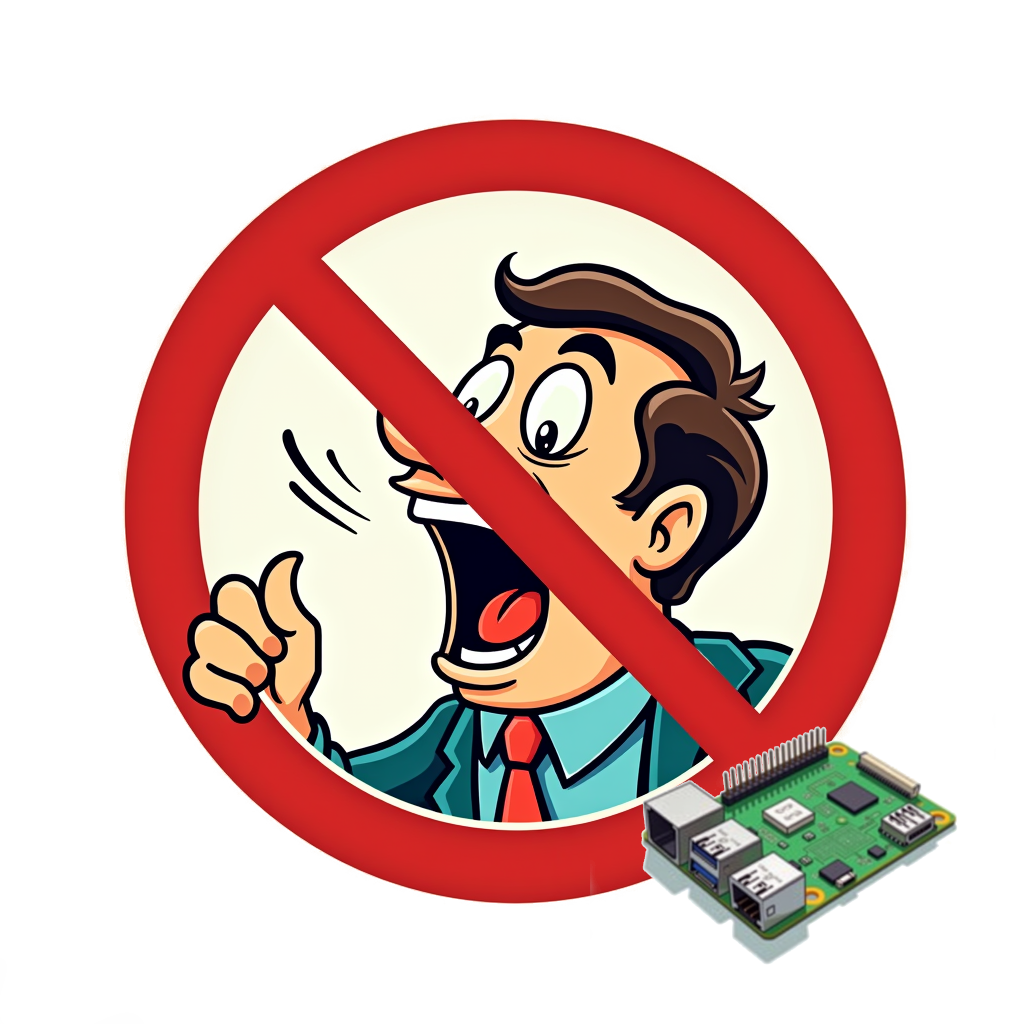
\includegraphics[scale=0.14]{Logo.png}}
	\end{center}
\end{frame}

\section{L'hardware}
\begin{frame}{L'hardware}
	\begin{itemize}
		\item Il sistema è composto da un powerbank, un \href{https://www.raspberrypi.com/products/raspberry-pi-3-model-b-plus/}{Raspberry Pi 3B+}, un gruppo di altoparlanti da 5W e la \href{https://it.wikipedia.org/wiki/PlayStation_Eye}{PlayStation Eye}.
		\item Il Raspberry Pi usa i microfoni della PlayStation Eye per monitorare il rumore ambientale. Se il volume supera una soglia, il dispositivo riproduce un effetto eco tramite gli altoparlanti.
	\end{itemize}
	\begin{center}
		\zoombox{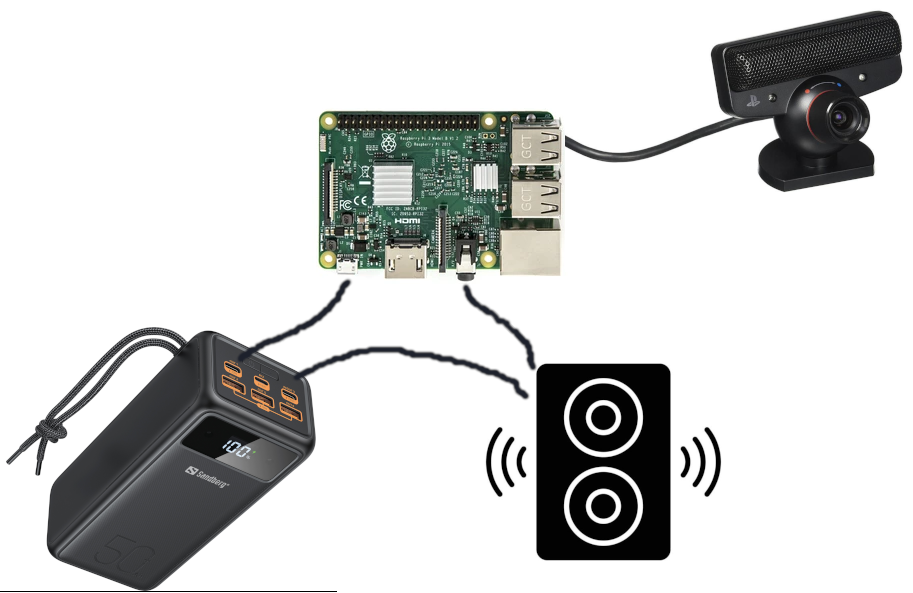
\includegraphics[scale=0.7]{schema.png}}
	\end{center}
\end{frame}

\section{Il software}
\begin{frame}{Il software}
	\begin{itemize}
		\item Il software principale, scritto in \href{https://www.python.org/}{Python}, monitora il rumore e attiva l’eco se necessario, registrando ogni evento e inviando i dati a \href{https://thingspeak.mathworks.com/}{ThingSpeak}.
		\item Una dashboard di controllo, realizzata con \href{https://www.python.org/}{Python}, \href{https://it.wikipedia.org/wiki/JavaScript}{JavaScript} e \href{https://nginx.org/}{Nginx}, è accessibile da browser e protetta da password.
	\end{itemize}
	\begin{center}
		\zoombox{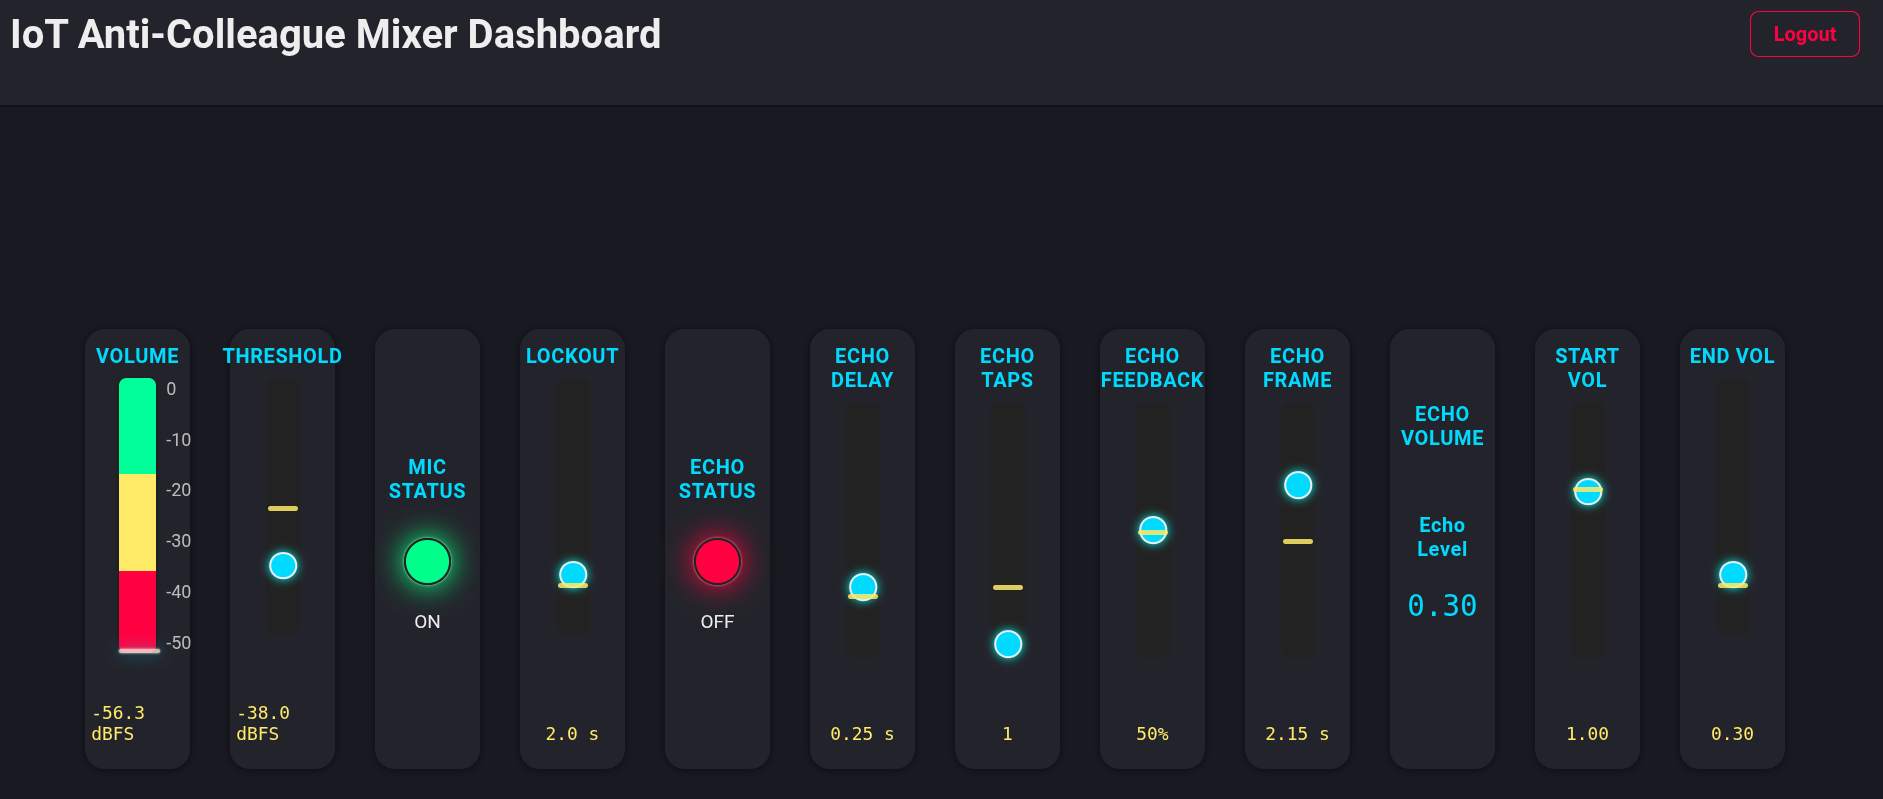
\includegraphics[scale=0.2]{mixer.png}}
	\end{center}
\end{frame}

\section{Sperimentazione sul campo}
\begin{frame}{Sperimentazione sul campo}
	\begin{tabularx}{\linewidth}{XX}
		{
			\centering
			\vspace*{-50mm}
			\begin{itemize}
				\item Il dispositivo è stato installato per due settimane nell’ufficio. I dati raccolti mostrano l’efficacia del sistema.
			\end{itemize}

		}&{
			\centering
			\zoombox{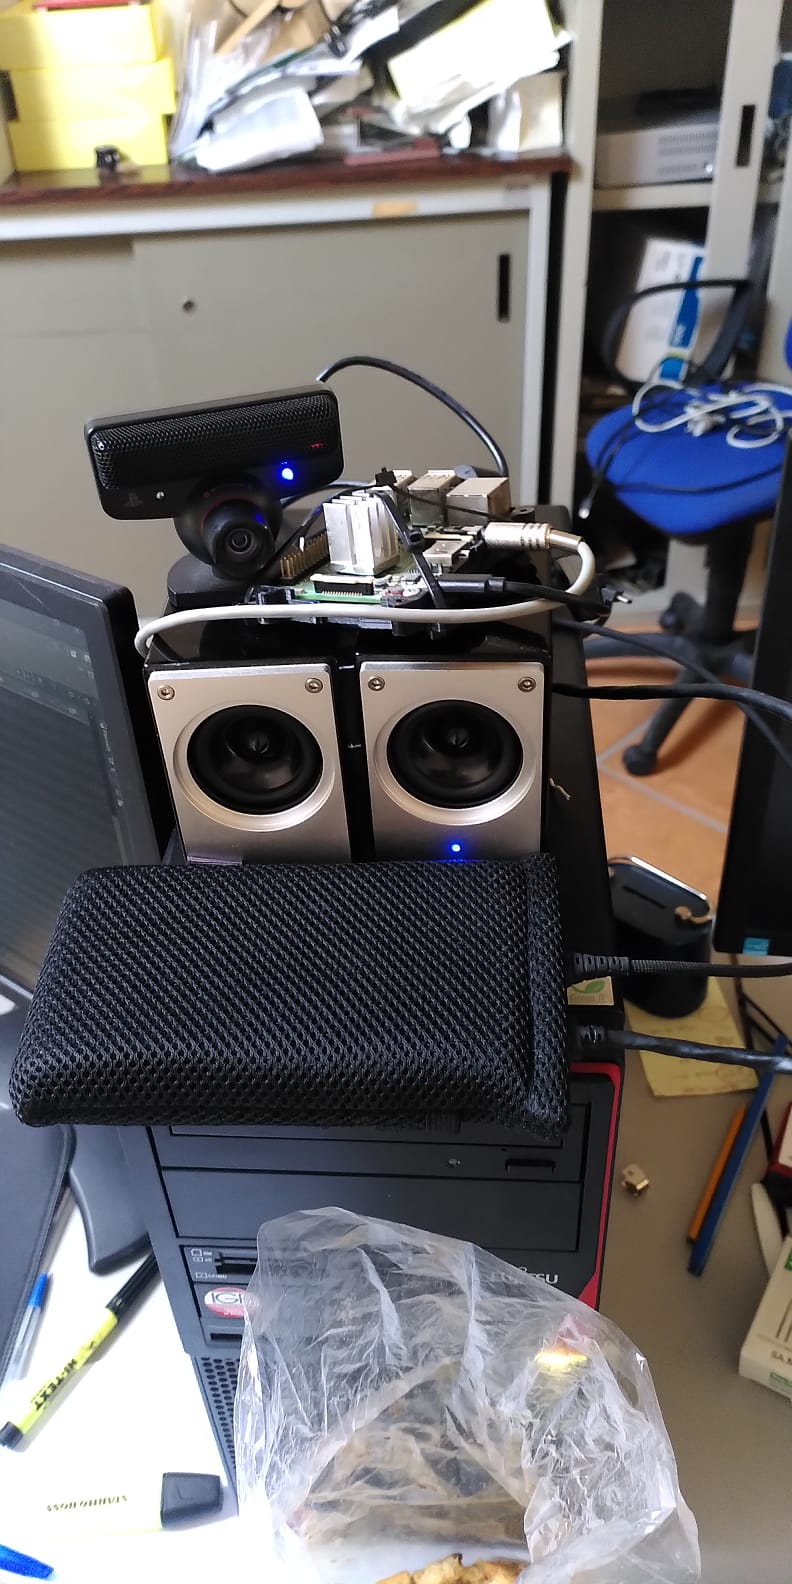
\includegraphics[scale=0.125]{work.jpeg}}
			
		}
	\end{tabularx}
\end{frame}

\section{Analisi dei dati}
\begin{frame}{Analisi dei dati}
	\begin{itemize}
		\item Durante le due settimane di test, il rumore provocato dai colleghi si è ridotto sensibilmente.
	\end{itemize}
	\vspace*{2mm}
	\begin{tabularx}{\linewidth}{XX}
		{
			\centering
			\zoombox{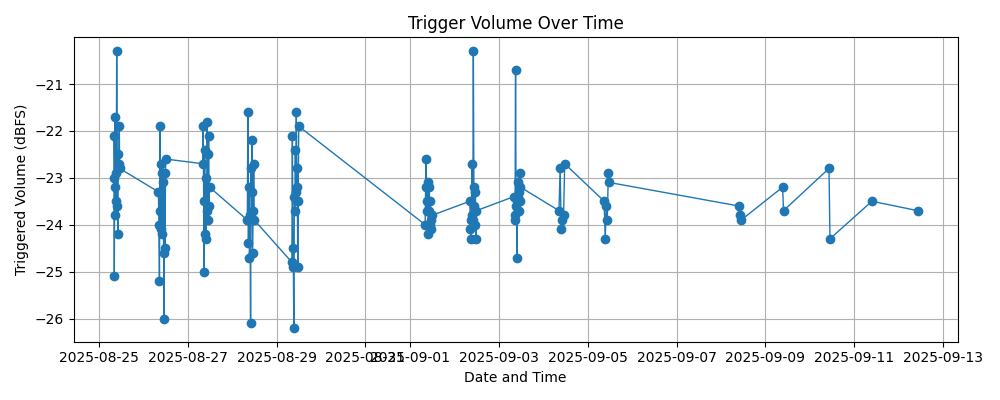
\includegraphics[scale=0.3]{trigger_volume_vs_time.png}}
			
		}&{
			\centering
			\zoombox{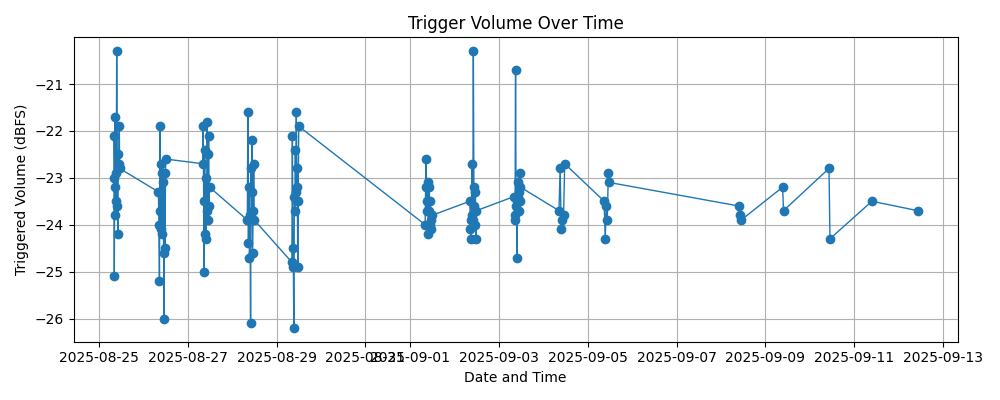
\includegraphics[scale=0.3]{trigger_volume_vs_time.png}}
			
		}
	\end{tabularx}
	
\end{frame}

\section{Valutazioni}
\begin{frame}{Valutazioni}
	\begin{itemize}
		\item Il sistema ha sensibilizzato i colleghi a mantenere toni di voce più consoni all’ambiente.
		\item Solo uno su otto colleghi ha percepito il dispositivo come troppo invasivo.
		\item In sintesi, il sistema si è dimostrato efficace nel ridurre il rumore e migliorare la collaborazione.
	\end{itemize}
\end{frame}

\section{Conclusioni}
\begin{frame}{Conclusioni}
	\begin{itemize}
		\item L’esperimento ha confermato l’efficacia del dispositivo.
		\item Tuttavia, l’utilizzo continuo dell’eco potrebbe risultare opprimente per chi lavora nell’ambiente.
		\item È consigliabile mantenere attiva solo la parte di monitoraggio e attivare l’eco solo se necessario, dopo aver avvisato i presenti.
	\end{itemize}
\end{frame}
	
\end{document}